\paragraph*{Quantifying Multistrain Communities}\mbox{}\\
For each community spread plate, the number of colonies of each composite phenotype were counted from photos. Ambient lighting environment slightly differed between treatments; we applied a small RGB scaling factor to low-nutrient environment photos to normalize differentiability between strains across treatments (R=1.11, G=1.09, B=1.05). Total number of colonies per plates was highly variable, a median number of colonies per plate of 161, but the overall range spanning from 5 colonies to 545. Figure \ref{fig:plateImages}. Plates were excluded from analysis if contamination obscured a large amount (<10\%) of the plate, or had low plate abundance (<5 colonies); \ref{tab:contamination_outcomes} shows the distribution of removed plates across treatments. 

\begin{figure}[h!]
  \begin{center}
    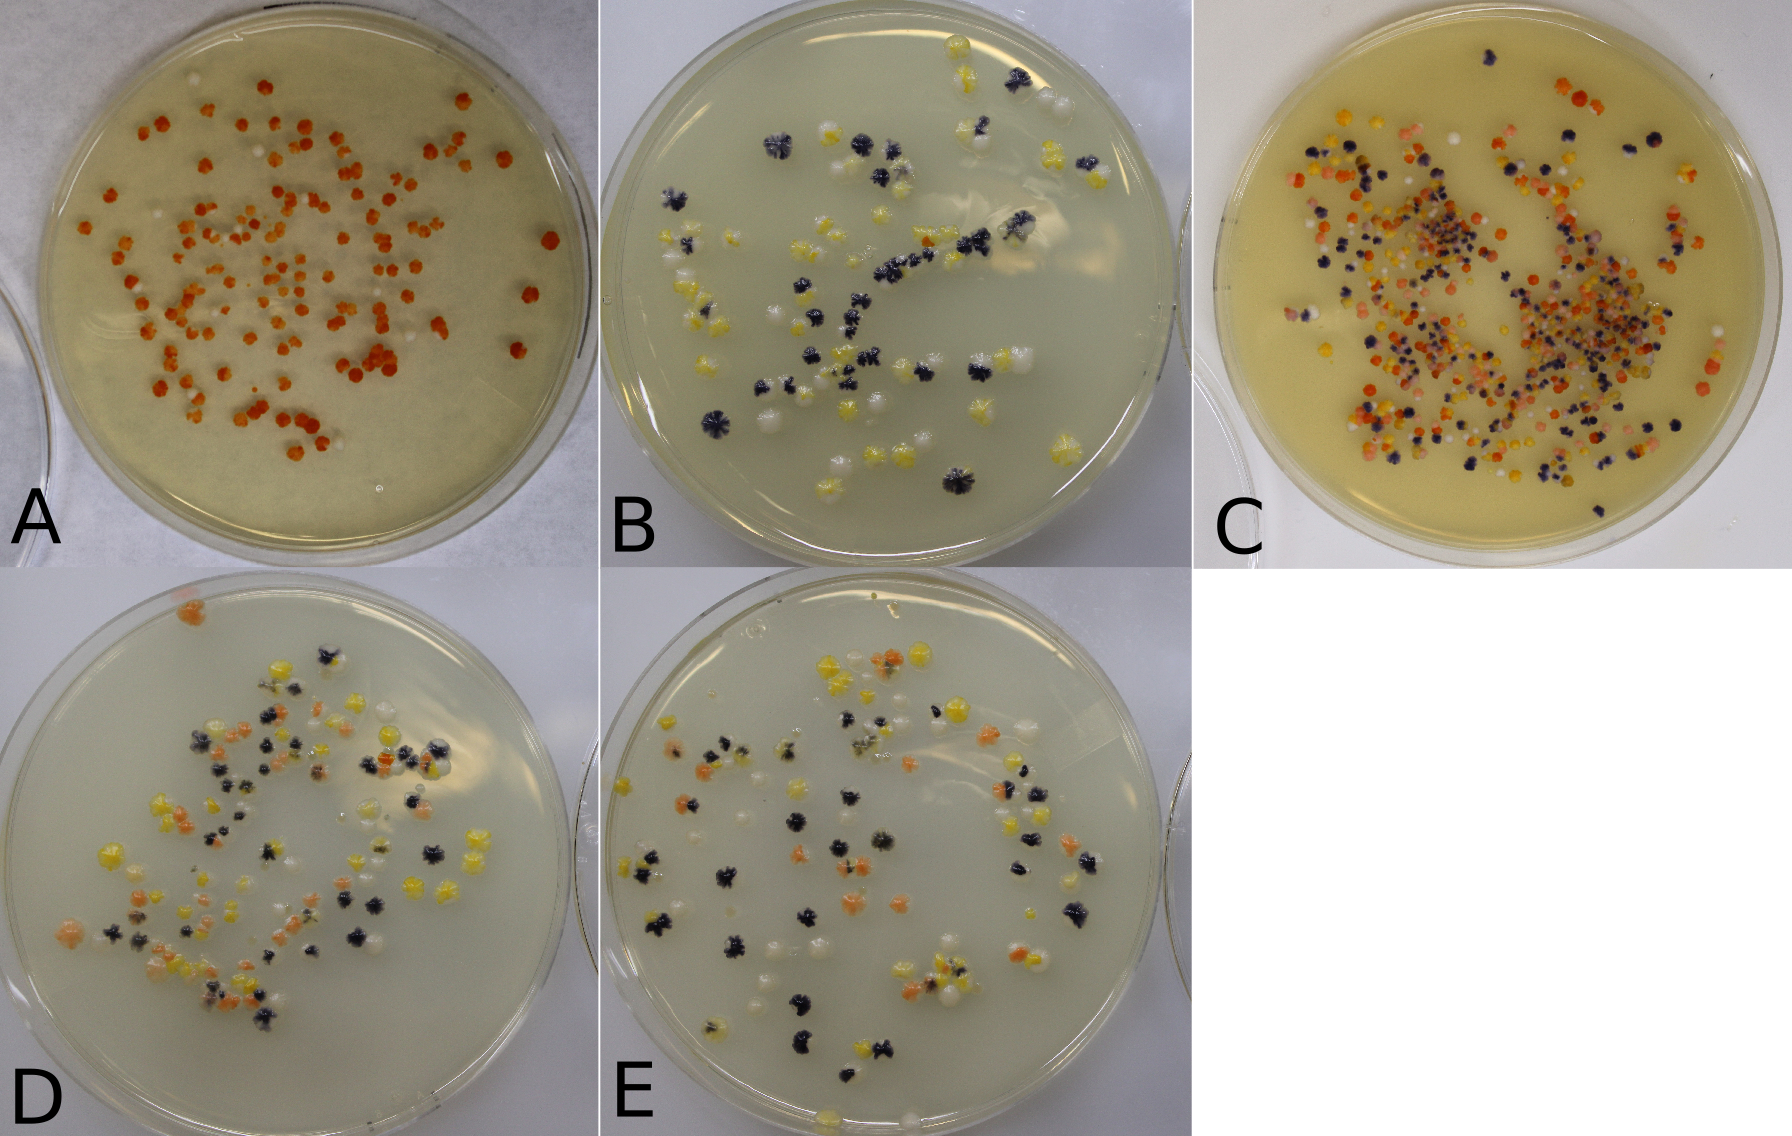
\includegraphics[width=\textwidth]{NutrientNeutrality/Figures/ExamplePlates.png}
    \caption[Example plates of community samples from a variety of replicates]{Example plates of community samples from a variety of replicates. Panels A, B, and C, represent samples of one-, two-, and four-strain communities, respectively. Panels D and E represent two samples of the same replicate three-strain community. Although experimental communities were inoculated only with colored strains, a minority of colonies did not express visible phenotypes and could instead appear wild-type appearing (mean = 15.2\% across strain-nutrient combinations), see \ref{fig:FullModel_CommunityBarcharts}.}
    \label{fig:plateImages}
  \end{center}
\end{figure}

Although experimental communities were inoculated only with colored strains, some colonies did not express visible phenotypes and could instead appear wild-type appearing. Because wild-type-appearing colonies in multispecies communities could originate from any strain present in the community, we used a Bayesian hidden-state model informed by monoculture expression rates and observed phenotype counts to estimate underlying strain relative abundances in each final community. 

We model the relative abundances within each community-treatment combination as a singular grand mean, with individual replicates deviating from this mean according to a replicate-level variance parameter. Individual plates are modeled as multinomial draws from replicate-level distributions, modified by the independently modeled strain-specific phenotype expression rates. As such, we are able to model the best-fit relative abundance distribution of each replicate given our our observed phenotypic counts, along with our estimates uncertainty around those relative abundances. We present the results of these modeled relative abundances in main text figure \ref{fig:CommunityBarcharts}. Visual comparisons of raw and modeled relative abundances are presented in \ref{fig:FullModel_CommunityBarcharts}.  

        
\begin{sidewaysfigure}[p]
  \centering
  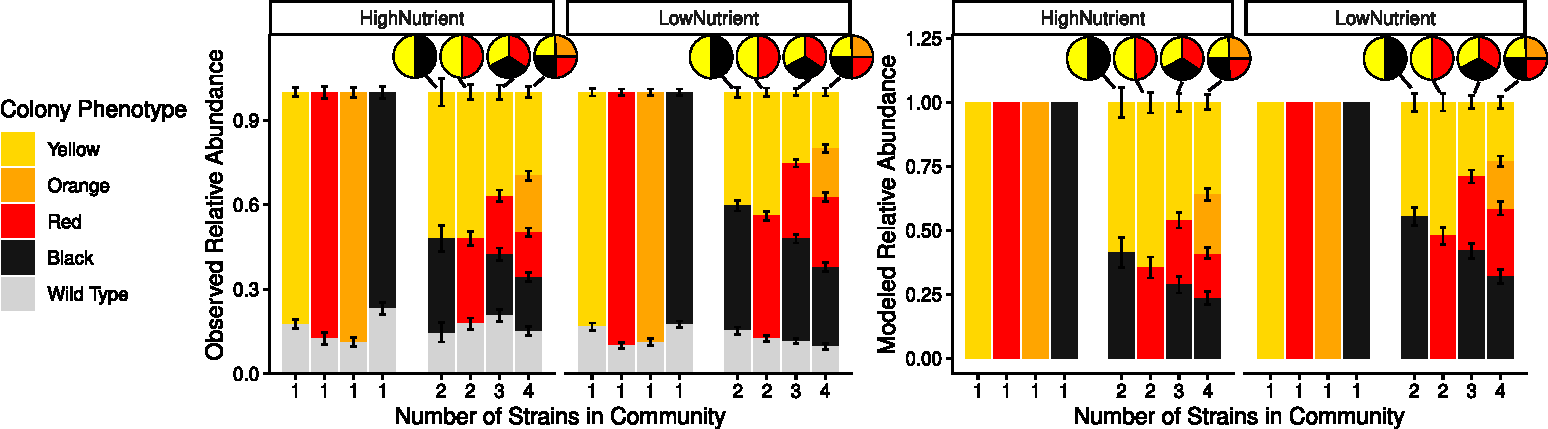
\includegraphics[width=\textheight]{NutrientNeutrality/Figures/CommunityBarcharts.pdf}
  \caption[Comparisons of observed and modeled relative abundance of strains across community compositions]{Relative abundance of strains across community compositions. Although experimental communities were inoculated only with colored strains, some colonies did not express visible phenotypes and could instead appear wild-type appearing. Because wild-type-appearing colonies in multispecies communities could originate from any strain present in the community, we used a Bayesian hidden-state model informed by monoculture expression rates and observed phenotype counts to estimate underlying strain relative abundances in each final community. The left panel shows observed colony phenotypes across community compositions, and the right panel shows inferred strain relative abundances.}
  \label{fig:FullModel_CommunityBarcharts}
\end{sidewaysfigure}





\begin{table}[ht]
\centering
\caption[Summary of successful replicates across community compositions and nutrient environments]{Summary of successful replicates across community compositions and nutrient environments. The experiment included eight community types grown in two nutrient environments, with eight replicates per community-environment combination. Each replicate was subsampled and spread-plated twice, yielding 256 total community samples. Samples were excluded from analysis if contamination obscured a large amount (<10\%) of the plate, or had low plate abundance (<5 colonies). For each community-environment combination, the table reports the number of biological replicates with two, one, or zero usable samples remaining after filtering. Across 128 community-environment replicates, 11 were fully excluded and 24 retained only one usable sample. These were generally spread relatively evenly community-environment combinations, with most excluding either one or zero replicates. The two exceptions are the high-nutrient yellow-black communities (3 replicates excluded) and low-nutrient yellow-red-orange-black communities (2 replicates excluded). 
}
\label{tab:contamination_outcomes}
\begin{tabular}{| l | c | c | c | c | c | c |}
  \hline
  \multirow{2}*{\textbf{Community}}
    & \multicolumn{3}{c|}{\textbf{High Nutrient}}
    & \multicolumn{3}{c|}{\textbf{Low nutrient}} \\
  \cline{2-7}
    & 2 samples & 1 sample & 0 samples & 2 samples & 1 sample& 0 samples\\
  \hline
  Yellow & 5 & 2 & 1 & 6 & 2 & 0 \\
  \hline
  Red & 4 & 3 & 1 & 6 & 1 & 1 \\
  \hline
  Orange & 5 & 3 & 0 & 6 & 2 & 0 \\
  \hline
  Black & 7 & 1 & 0 & 7 & 1 & 0 \\
  \hline
  Yellow-Black & 4 & 1 & 3 & 8 & 0 & 0 \\
  \hline
  Yellow-Red & 5 & 2 & 1 & 6 & 1 & 1 \\
  \hline
  Yellow-Red-Black & 6 & 2 & 0 & 7 & 0 & 1 \\
  \hline
  All strains & 7 & 1 & 0 & 4 & 2 & 2 \\
  \hline
\end{tabular}
\end{table}
\newpage
\paragraph*{Monoculture Growth Curves}\mbox{}\\
We estimated strain-specific vital by growing each strain in liquid monocultures. Figure \ref{fig:growthCurves} shows the example demographic curves used to fit a logistic model, such

\begin{equation}
    N_{n,t+1}=N_{n,t}+R_nN_{n,t}\left(1-\frac{N_{n,t}}{K_n}\right)
\end{equation}

The finite rate of increase (R) and carrying capacity (K) were estimated separately for each strain-by-nutrient combination; each timestep of our discrete model represented a 10 minute interval between OD600 measurements. Replicate trajectories were allowed to vary in R around their corresponding strain-by-nutrient mean, with a single replicate-level variance parameter shared across all groups. Observation error was modeled with a shared lognormal error term, and weakly informative priors were placed on log-transformed vital-rate parameters and variances. Models were fit using four MCMC chains with 1000 timesteps following a 1000-timestep burn-in period. Models were checked for convergence by analyzing ESS and $\hat{R}$ for each parameter estimate, as well as through posterior predictive visualizations. Though with high variability, we observed a potential negative trade-off between R and K across strains in both high- and low-nutrient treatments (Figure \ref{fig:Sup_RvsKscaling}).




\begin{figure}[h!]
  \begin{center}
    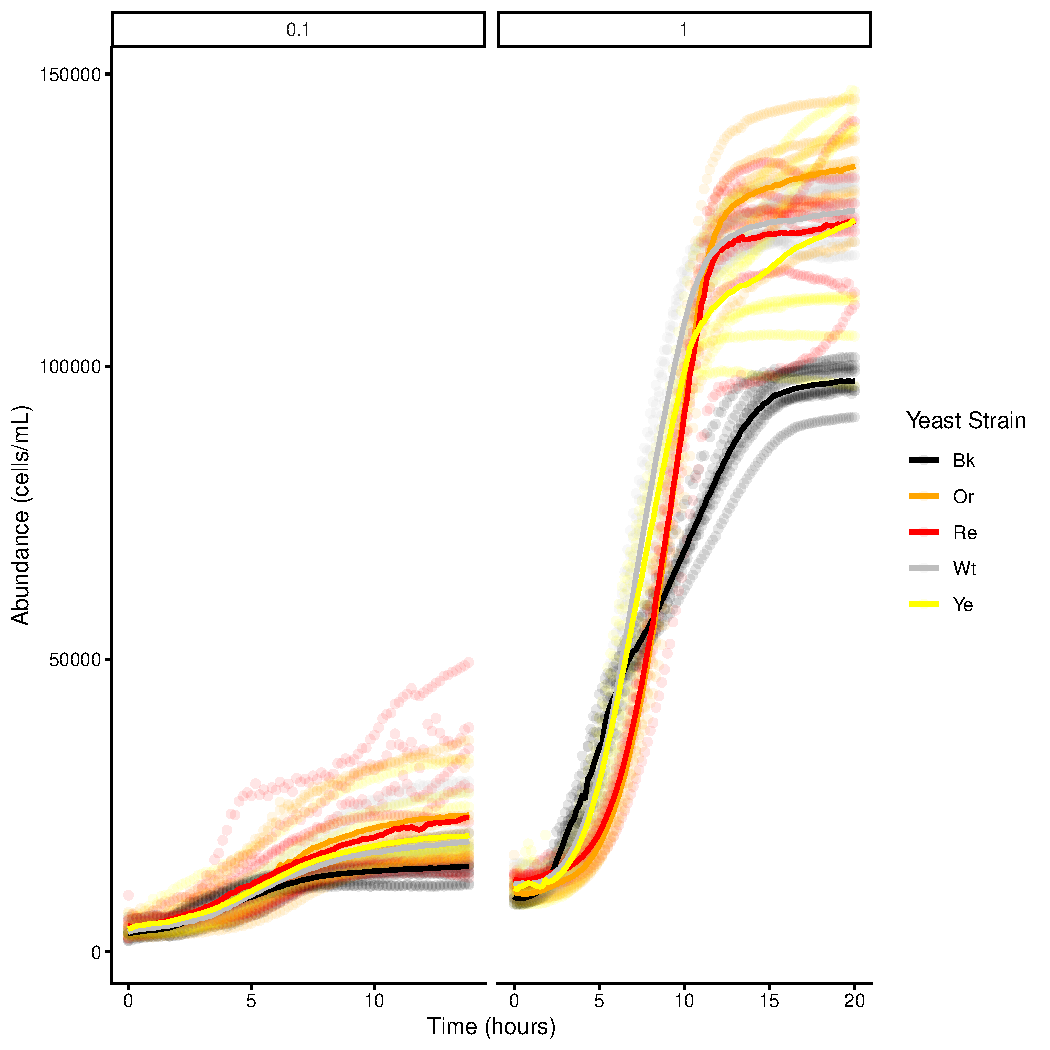
\includegraphics[width=\textwidth]{NutrientNeutrality/Figures/growthCurves.pdf}
    \caption[Monoculture growth curves used to inform vital rate estimates]{Monoculture growth curves used to inform vital rate estimates. Density if measured through transforming optical density measurements to cellular density via standard curves. Left and right panels represent low and high-nutrient conditions. Points represent individual culture trajectories, while lines represent mean values across all replicates.}
    \label{fig:growthCurves}
  \end{center}
\end{figure}



\begin{figure}[h!]
  \begin{center}
    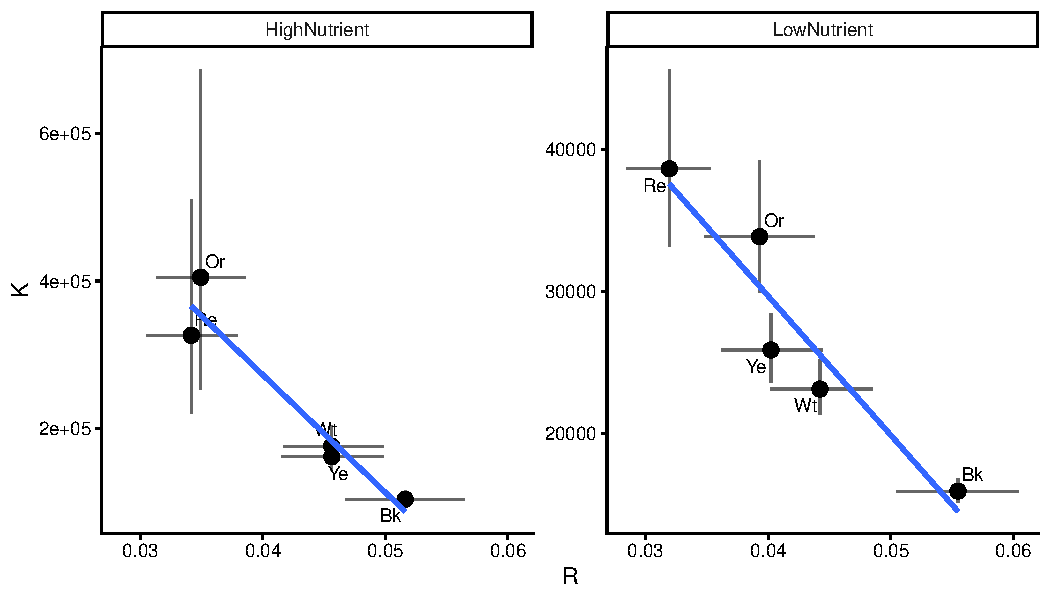
\includegraphics[width=\textwidth]{NutrientNeutrality/Figures/Sup_RvsKscaling.pdf}
    \caption[Comparison of best fit carrying capacity (K) and finite rate of increase (R) values across nutrient environment]{Comparison of best fit carrying capacity (K) and finite rate of increase (R) values across nutrient environment. Error-bars represent 95\% credible intervals. We observe a significant negative relationship between the two parameters across both nutrient environments. }
    \label{fig:Sup_RvsKscaling}
  \end{center}
\end{figure}

